\documentclass[notitlepage]{report}
\usepackage[left=1in, right=1in, top=1in, bottom=1in]{geometry}

\usepackage{titling}
\usepackage{graphicx}
\usepackage{fullpage}
\usepackage{algorithm}
\usepackage{amsfonts}
\usepackage[noend]{algpseudocode}

\pretitle{\begin{center}\Huge\bfseries}
\posttitle{\par\end{center}\vskip 0.5em}
\preauthor{\begin{center}\Large\ttfamily}
\postauthor{\end{center}}
\predate{\par\large\centering}
\postdate{\par}

\title{A Brief Dive into Graph Isomorphism}
\author{Kevin Richard Koch}
\date{\today}
\begin{document}

\maketitle
\thispagestyle{empty}

\begin{abstract}
In this paper I will explain my exploration of graph isomorphism as a problem in computer science, as well as an algorithm I discovered written by Ullmann in 1976. The algorithm explores a subset of the graph isomorphism problem, sub graph isomorphism. I will also go into some of the real world applications of Graph Isomorphism, as well as the history and future for the topic.
\end{abstract}

\section*{What is graph isomorphism}
Graph Isomorphism, here after refereed to as GI, is a characteristic of a graph to be able to be rewritten in different ways, while still maintaining the same information.
\begin{figure}[h!]
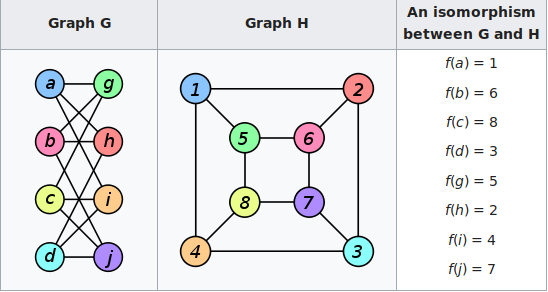
\includegraphics[width=\linewidth]{/home/cptwalmart/Documents/COSC320/Graph-Isomorphism-Project/images/WikiGraphIsomorphismExample.png}
\caption{An example of an isomorphic graph}
\end{figure}

As you can see from the two graphs, even though they look very dissimilar, they are infarct the same graph. This property is extremely useful in many fields today. Chemists are able to look at the molecular makeup of different substances, and use GI to identify known atomic structures. This aspect of GI is so researched in fact that it is known as the "Chemist's Problem".

I should also take a moment to address what exactly is the Graph Isomorphism problem. Suppose that $\omega^{1}$ and $\omega^{2}$ are two graphs with $n$ vertices, the GI problem asks if they are isomorphic or not. GI plays an important role in Computer Theory because it lies in the class known as NP, and is rated NP-Hard. It is unknown if it lies in P or NP-Complete, however most heuristic evidience stronly implies that it is not NP-Complete. Further evidence of this is the fact that if it was proven that this is NP-Complete, then the polynomial hierarchy would collapse. GI is known to be polynomial complete for graphs of bounded degree, bounded genus, bounded eigenvalue mutiplicity, and treewidth. The problem of counting the number of isomorphisms between two graphs is Turing reducible to the inversion of the graph itself. It is known that it has a time complexity of at most exp$(O(n^{2/3}))$ for a graph with V(n). Also there are plenty of general algorithms for GI wheich are "practical in practice" meaning there are some worst case inputs which cause it to have a horrendius run time, however for most it is fine.  ~\cite{derksen, hartke}


Now before we continue, I should define some terminology so it is known when referenced later on in the paper. A graph through this paper shall be known as an \textit{combinatorial graph}. So, a graph G is a finite set of \textit{vertices} plus a set of ordered or unordered pairs of vertices named \textit{edges}. A set of vertices shall be noted as \textit{V(G)} while a set of edges will be noted as \textit{E(G)}. Graphs containing ordered pairs shall be known as \textit{directed} and ones with unordered pairs shall be known as \textit{undirected}. Graphs shall be assumed to be undirected unless otherwise noted. The number of edges of a vertex shall be known as a \textit{valence} of the vertex. For a vertex, the number of head ends adjacent to a vertex is called the \textit{indegree} of the vertex and the number of tail ends adjacent to a vertex is its \textit{outdegree}. (How many nodes point to it, and how many point out.) A \textit{connected component} is a subgraph in which any two vertices are connected to each other by paths, and which is connected to no additional vertices in the supergraph. A \textit{loop} is an edge that connects a vertex to itself. And finally a \textit{parallel edge} are two or more edges which are incident to the same two vertices.

\subsection*{Properties of Graph Isomorphism}
For a graph to be isomorphic, it must fulfill several criteria. Not every graph that looks similar are isomorphic, one key feature of an isomorphic graph is that $V^{1}(G) = V^{2}(G)$, and $E^{1}(G) = E^{1}(G)$. There must exist a one to one mapping between the graph's vertices, and the following properties are satisfied, then the two graphs are said to be isomorphic.

\begin{enumerate}
\item $V^{1}(G) = V^{2}(G)$
\item $E^{1}(G) = E^{1}(G)$
\item The indegree and outdegree should be equal
\item The number of connected components should be the same
\item The number of loops should be the same
\item The number of parallel edges should be the same
\end{enumerate}

\subsection*{The Chemist's problem}
This problem is actually identifying what molecule is what. Say you're given the molecule for water, which is commonly known as H$_{2}$O. You would have to analyze different structures and try and match it with water. So efficient graph isomorphism algorithms are super convenient here, since molecules can be made into a graph form where the bonds would be the edges, and the vertexes would be the different atoms that make up the compound.~\cite{miller}

Miller then goes on to describe a process  where he determines certificates for different equivalence relations. A certificate is defined as a graph that has an isomorphism, and a deterministic certificate if $f$ is a certificate and is computable in polynomial time. Further, a succinct certificate is a certificate which is computable in NP time. This brings us to an open question presented in the article of what is the relation of the following four properties other than 1 implies 2 implies 4 and 1 implies 3 implies 4:

\begin{enumerate}
\item $<A,\equiv>$ has deterministic certificates.
\item equivalence of $A$ over $\equiv$ is in $P$.
\item $<A,\equiv>$ has succinct certificates
\item equivalence of $A$ over $\equiv$ is in $NP \cap \overline{NP}$
\end{enumerate}
(where $\equiv$ is an equivalence relation over a set $A$).

It is not known (as of this paper)if graph isomorphism satisfies any of the above four conditions. Sine polynomial time reduciability preserves all of the conditions, a positive solution for graph isomorphism would imply a positive solution for structures. In fact, graph isomorphism isn't known to satisfy any of the above conditions. This again leads us back to the discussion of isomorphism was found to be polynomial reducible, all the classes would fall apart.~\cite{miller}

\section*{The Algorithms}
In researching graph isomorphism, I discovered that there is a multitude of different facets of the graph isomorphism problem, and I was overwhelmed with the plethora of options out there for me to research, so I ended up taking a bit of a shotgun approach, studying graph isomorphism as a broad topic, then diving deeper into some of the sub problems that come as a result of graph isomorphism. I read in one of the papers that graph isomorphism gained so much popularity within the computer science fields when it was first being researched that it was even referred to as the "four-color disease".~\cite{read}

So my research eventually lead me to the following brute force algorithm. Included is the unaltered version of their algorithm, later on I will show my changes.

So a brute force algorithm for graph isomorphism, is exponential in the amount of time it takes to process. The following algorithm has a run time of $O(N^{2}-N!)$ where n is the number of vertices in the two graphs we test on. The procedure is simple, enumerate and test all permutations of the vertices of one of the two graphs(in this case graph 2), until an isomorphism mapping is found. If it exhausts every possible permutation then the two graphs are not isomorphic. Notes for the following algorithms, the boolean array 'used' marks which vertices have been mapped. The array perm records the vertex mapping. For all $V\in$G1, perm[x] contains the label of the mapped vertexes in G2.~\cite{tolley}

\begin{algorithm}
\caption{BruteForceWrap}
\begin{algorithmic}[1]

\Procedure{BruteForceWrap}{}
    \State isomorphic = BruteForce(N-1) \Comment{calls upon brute force to find if isomorphic is true or false}
    \If{$isomorphic = TRUE$}
        \State write "Graphs are Isomorphic."
    \Else
    	\State write "Graphs are not Isomorphic."
    \EndIf
    \label{A1}
\EndProcedure
\end{algorithmic}
\end{algorithm}

\begin{algorithm}
\caption{Brute Force}
\begin{algorithmic}[1]

\Procedure{BruteForce}{$level$}       
    \State result = FALSE 								
    \If{$level = -1$}									
    	\State result = CheckEdges($G$)
    \Else
    	\State i = 0
	    \While{$i < N$ \& $result = TRUE$}				\Comment{Runs until you run out of vertexes or you find a match}
        	\If{$used[i] = FALSE$}
	        	\State used[i] = TRUE 					\Comment{keeps track of what nodes you've visited during recursion}
	        	\State perm[level] = i
	        	\State result = BruteForce($level - 1$)
	        	\State used[i] = FALSE					\Comment{Resets state after we are done with it}
	        \EndIf
	        \State i = i + 1	
	    \EndWhile
	\EndIf
	\State return result
\label{BruteForce}
\EndProcedure

\end{algorithmic}
\end{algorithm}

\begin{algorithm}
\caption{Check Edges}
\begin{algorithmic}[1]

\Procedure{CheckEdges}{}       
    \State diff = TRUE
    \For{$x = 0$ to $N-1$}
        \State y = 0
        \While{$y < N$ \& $diff = FALSE$}
        \If{$adj\_matrix1[x][y] \neq adj\_matrix2[perm[x]][perm[y]]$} 
        	\State diff = TRUE
        \EndIf
        \State y = y + 1
        \EndWhile
    \EndFor
    \State return diff
\label{CheckEdge}
\EndProcedure

\end{algorithmic}
\end{algorithm}
\newpage

So this algorithm proved quite troublesome for me. I can only assume the original authors were erroneous and lax in their checking of it before their submission. The first thing the astute will notice is that, as written the code will not ever go into one of the loops. Fixing this proved quite troublesome for me, but eventually I was able to find the correct set of boolean values to parse the algorithm successfully. Secondly, the algorithm has no accounting for the 'base case' which is that the two graphs are identical. Finally, I decided to beef up the algorithm slightly, accounting for two of the six properties of Graph Isomorphism, the number of edges and the number of vertices. These were the easiest of the properties to implement and if I return to researching this topic, I will take more care to handle these cases.

\begin{algorithm}
\caption{Brute Force Wrap - Kevin Edit}
\begin{algorithmic}[1]

\Procedure{BruteForceWrap}{}
    \State sanity = SanityCheck()
    \If{$!sanity$}
    	\State Exit
    \EndIf
    \State isomorphic = TwinCheck()
    \If{$isomorphic$}
    	\State The graph is isomorphic! Exit
   	\EndIf
   	\State isomorphic = BruteForce(N-1)
    \If{$isomorphic = TRUE$}
        \State write "Graphs are Isomorphic."
    \Else
    	\State write "Graphs are not Isomorphic."
    \EndIf
    \label{A2}
\EndProcedure
\end{algorithmic}
\end{algorithm}

\begin{algorithm}
\caption{Brute Force-Kevin Edit}
\begin{algorithmic}[1]

\Procedure{BruteForce}{$level$}       
    \State result = FALSE 								
    \If{$level = -1$}									
    	\State result = CheckEdges($G$)
    \Else
    	\State i = 0
	    \While{$i < N$ \& $result = FALSE$}				\Comment{Runs until you run out of vertexes or you find a match}
        	\If{$used[i] = FALSE$}
	        	\State used[i] = TRUE 					\Comment{keeps track of what nodes you've visited during recursion}
	        	\State perm[level] = i
	        	\State result = BruteForce($level - 1$)
	        	\State used[i] = FALSE					\Comment{Resets state after we are done with it}
	        \EndIf
	        \State i = i + 1	
	    \EndWhile
	\EndIf
	\State return result
\label{BruteForce2}
\EndProcedure

\end{algorithmic}
\end{algorithm}

\begin{algorithm}
\caption{Check Edges-Kevin Edit}
\begin{algorithmic}[1]

\Procedure{CheckEdges}{}     
    \State same = TRUE
    \For{$x = 0$ to $N-1$}
        \State y = 0
        \While{$y < N$ \& $same =$ TRUE}
        \If{$adj\_matrix1[x][y] \neq adj\_matrix2[perm[x]][perm[y]]$} 
        	\State same = FALSE
        \EndIf
        \State y = y + 1
        \EndWhile
    \EndFor
    \State return diff
\label{CheckEdge2}
\EndProcedure

\end{algorithmic}
\end{algorithm}



\begin{algorithm}
\caption{TwinCheck}
\begin{algorithmic}[1]

\Procedure{TwinCheck}{}     
    \State same = TRUE
    \For{$x = 0$ to $N-1$}
        \State y = 0
        \While{$y < N$ \& $same =$ TRUE}
        \If{$adj\_matrix1[x][y] \neq adj\_matrix2[x][y]$} 
        	\State same = FALSE
        \EndIf
        \State y = y + 1
        \EndWhile
    \EndFor
    \State return diff
\label{CheckEdge3}
\EndProcedure

\end{algorithmic}
\end{algorithm}

\begin{algorithm}
\caption{Sanity}
\begin{algorithmic}[1]

\Procedure{Sanity Check}{}     
    \If{$vert1!=vert2$}
    	\State return false
    \ElsIf{$edge1!=edge2$}
    	\State return false
    \Else
    	\State return true
    \EndIf
\label{SanityCheck1}
\EndProcedure

\end{algorithmic}
\end{algorithm}
\newpage

Due to the exponential time of this brute force algorithm and the time I had remaining, I wasn't able to test very high node counts. Also I noticed when I ran my tests with a system clock check, they took far less time than when I tried to run it to just ensure the program worked. Is it possible that there was a background operation that caused my tests to 'complete' too quickly? I'm unsure and wish I had given myself more time to investigate this further. In  addition, it wasn't until late in my research I discovered the paper that I based my algorithm on. I had been looking at several other papers and resources for writing this report. Regardless, I discovered a DFS algorithm that would have been enjoyable to implement and test against the brute force method. Looking at the the research from Tolley, Franceschini, and Petty, it looks as though they were able to test the three algorithms to upto a hundred nodes, and the DFS algorithm crushed the other's they tried.~\cite{tolley}

\section*{Closing Thoughts}
Graph isomorphism has and will continue to be one of computer science's 


\bibliography{bib}
\bibliographystyle{plain}


\end{document}